\chapter{DMD applied to the IL-10-GAG system}

The previous chapter presented Dynamic Molecular Docking (DMD), a novel
molecular dynamics-based local docking method well-suited for exploring
protein-GAG interaction. I applied DMD to the IL-10-GAG system, using the
binding region prediction derived in \cref{chapter:bspred}. The goal was to
further characterize the interaction of GAGs with IL-10 in that region, and to
identify potential molecular mechanisms of IL-10-GAG interaction. This chapter
seeks to present \textit{i)} the computational challenges, \textit{ii)} the
methodological details, and \textit{iii)} the major outcomes of this endeavor.

Several DMD studies were performed, with varying DMD parameterization as well as
varying molecular system setup. Conducting these studies required an increment
of the computational resources available to us by orders of magnitude. In the
course of performing these studies I continuously refined the software
architecture for controlling the corresponding high performance computing
resources and enriched the DMD data analysis framework, as described in this
chapter. One of the main results of the IL-10-GAG DMD studies presented here is
the identification of IL-10's R107 as key residue for GAG binding.


\section{Methods}

\subsection{Computational framework}

With the standard high performance computing resources available in Dresden, the
conduction of DMD studies required for IL-10-GAG investigation would not have
been possible. Hardware and software engineering was required in order to
develop a system architecture that allowed for efficient conduction of DMD
studies. This subsection provides technical information about these engineering
decisions.

\subsubsection{High performance computing requirements of one DMD study}

One DMD study according to the protocol as presented in \cref{chapter:dmd},
i.e.\ with $N = 100$ repetitions, a pulling process simulation time of
\SI{4}{\nano\second} and a free MD simulation time of \SI{10}{\nano\second}
implicates about \SI{1.4}{\micro\second} of simulated real time. As of these
numbers, one DMD study requires about 12 years ($10^5$ hours) of accumulated CPU
time using state-of-the-art hardware (such as the Intel Xeon Processor X5650).

In high performance computing (HPC), computational tasks are usually abstracted as
\enquote{jobs}, whereas a job is a sub-problem of an \enquote{embarrassingly
parallel} problem \cite{heath1986hypercube}, for which little or no effort is
required to separate the problem into a number of independent tasks. For
efficient use of HPC batch schedulers for DMD, I have abstracted a DMD study
into the following list of jobs (whereas some of the jobs named later in the
list require completion of those listed earlier):

\begin{itemize}
\item LROM system preparation jobs (minimization, heat-up, equilibration)
\item $N$ tMD production jobs
\item $N$ free MD jobs (minimization, heat-up, equilibration, production)
\item $N$ final state validation and energy minimization jobs
\item $N$ free MD trajectory analysis jobs (MM-PBSA)
\item $N$ free MD trajectory analysis jobs (MM-GBSA + SRED)
\item $N$ free MD trajectory analysis jobs (geometry and hydrogen bonding
analysis)
\end{itemize}

Depending on $N$, this yields on the order of $10^3$ computing jobs per DMD
study. The raw data created by those jobs comprises on the order of $10^2$
gigabytes distributed in about $10^5$ files.


\subsubsection{Establishment of GPU computing resources}

Initially, the execution of a single DMD study lasted about three weeks, using
the \enquote{Atlas} resource pool (provisioning a large number of AMD Opteron
6274 CPUs) in the supercomputing center of the TU Dresden (ZIH). However, this
system was affected by various technical issues and did not reliably allow us to
perform multiple DMD studies in parallel, or even increase the number of DMD run
repetitions $N$. The computational capacity of the in-house computing cluster of
the BIOTEC, TU Dresden (the \enquote{biocluster}, comprised of about 30
machines) was insufficient for performing DMD studies.

For mitigating issues related to a lack of computing resources for DMD, and
especially for the IL-10-GAG system investigation via DMD, our research group
became early adopter of a new HPC technology: the usage of graphics processing
units (GPUs) for general purpose computing (\enquote{GPGPU}
\cite{wikipedia_gpgpu}). Simply spoken, GPUs make heavy use of the so-called
single instruction, multiple data paradigm (SIMD, see
\cite{kirk2012programming_gpus} for further information), which matches common
algorithms used in MD simulations very well. That is, MD simulations can take
strong advantage of GPU hardware architectures. Compared to classical computing
architectures, this leads to \textit{i)} a significantly higher absolute
simulation performance (measured in nanoseconds of simulated time per day) and
\textit{ii)} a much better performance per financial cost ratio, considering
acquisition cost as well as energy cost. With the MD simulation framework Amber
12 \cite{case_amber_12} and corresponding patches
\cite{amber_12_patches}, the Amber developers were among the first to work on
and release a solid and efficient MD implementation for GPUs (pmemd.cuda, see
\cite{amber_gpu_2012,amber_gpu_pme_2013} for methodological details and
validation).

Correspondingly, I built up a GPU computing cluster in our research group, which
required substantial amounts of planning and testing, because no
enterprise-level vendors were available for this kind of hardware. Hence, this
cluster was composed based on raw hardware and software components, eventually
yielding the following configuration:

\begin{itemize}
\item Four dedicated compute nodes, based on low-clocked Intel central
processing units (CPUs) on special consumer-level mainboards, placed in
temperature-regulated server racks.
\item A total of 15 GPU devices distributed among these machines (2 Tesla C2070,
3 GTX 580, 2 GTX 690, 4 GTX 770, 4 GTX TITAN, all Nvidia CUDA devices
\cite{nvidia_cuda_devices}, purchased in batches spread across 1.5 years).
\item Linux operating systems, along with appropriate drivers and CUDA runtime
libraries.
\item A customized Torque \cite{torque_website} GPU job scheduling system, see
\cite{gehrcke_torque_gpu_setup} for details.
%\item pmemd.cuda, built
\end{itemize}

With this infrastructure at hand, I was able to perform a single DMD study
within less than two weeks, without being dependent on \textit{external}
resources. On top of that, from summer 2013 on I have been part of the testing
period of the large-scale GPU computing cluster of the supercomputing center of
the TU Dresden: as a section of their \enquote{Taurus} platform, they provide 80
Nvidia CUDA GPU devices (Tesla K20X). All in all, with these GPU resources at
hand, I was able to perform single DMD studies on a weekly basis, with a
significantly increased number of DMD runs per study ($N=200$ or $300$). In
Dresden, this would not have been possible using classical computing resources.


\subsubsection{Software architecture}

Above, it was stated that one DMD study is comprised of $\mathcal{O}(10^3)$
computing jobs, and that it requires storing hundreds of gigabytes of raw data
distributed in $\mathcal{O}(10^5)$ files. These numbers suggest that the
management of corresponding jobs and data requires a well-engineered controlling
system. The essential purpose of such system is to automatically identify errors
and recover from those: the likelihood for a single computing machine to fail
times the number of machines involved in a DMD study integrated over the
computing time yields a significant probability for the study to be affected by
\textit{one or more} technical issues. In other words, there is a guarantee that
something goes wrong. By experience I can tell that this prediction came true,
and manual identification of corresponding issues was a daunting task, which is
why I iteratively developed a system architecture that enables the efficient
conduction of DMD studies.

One requirement for this management architecture was to support all involved
hardware platforms, i.e.\ the Taurus GPUs, the Taurus CPUs (for data analysis),
the group-internal GPU cluster, and the biocluster CPUs (for data analysis).
These platforms involve three different batch scheduling systems. As all of
these platforms are based on POSIX-compliant operating systems with reliable and
well-performing file systems attached, I abstracted the data structure for
managing and monitoring a DMD study on top of the file system hierarchy, and
implemented basic data creation, manipulation, and validation using
well-established POSIX command line tools, incorporated in shell scripts.

For many purposes of data validation and analysis I implemented Python
programs based on Biopython \cite{biopython_web} and SciPy/NumPy
\cite{scipy_numpy} whenever appropriate. Data plotting was performed using
the Python module Matplotlib \cite{matplotlib_web}. Iterative development and
continuous integration of this software architecture was largely facilitated by
the efficient usage of a decentralized version control system (Mercurial
\cite{mercurial_web} in this case). For reference, the corresponding code
repository is available at \url{http://bit.ly/jgehrcke-phd-dmd-control}.


\subsection{Overall study design}
\label{dmdil10:overallmethod}

As a reminder, the term DMD study covers many DMD run repetitions followed by
data analysis. Hence, within a single DMD study the \textit{constants} are ---
among others --- the chemical configuration of the ligand molecule and the
geometrical DMD parametrization, i.e.\ the protein core atom and the focus
point. Clearly, a systematic investigation of the IL-10-GAG system via DMD
requires \textit{variation} of exactly these entities. Consequently, the planned
investigation requires the conduction of \textit{many} DMD studies. Initially,
the conduction and analysis of a single study consumed about two weeks. That is,
time and computational resources were the main limiters of the extent of this
endeavor. Hence, the goal was to get as much conclusive output out of as few DMD
studies as possible.

\subsubsection{Factors to investigate}

The entities that are obviously interesting to vary among the different DMD
studies in case of the IL-10-GAG system are:

\begin{itemize}

\item[1)] \textbf{The DMD protocol.} In the course of performing various DMD
studies I aimed for slight protocol changes for optimizing the computational
efficiency of DMD, compared to the protocol initially developed for the DMD
validation study described in \cref{chapter:dmd}. We decided to potentially
optimize parameters such as decreasing the tMD simulation length as well as the
LROM displacement length, both of which have direct impact on the pulling
process velocity. A the same time, I tried to increase the number of
independent DMD run repetitions within single DMD studies as far as our
computational resources allowed to, in order to obtain as much sampling
performance as possible.

\item[2)] \textbf{The geometrical DMD parameterization.} In
\cref{chapter:bspred}, a putative IL-10-GAG binding region was derived, which
can directly be used as input for designing IL-10-GAG DMD studies. For
potentially discovering a distinct and well-defined binding \textit{site} and
for investigating and finally eliminating the impact of the geometrical DMD
parameterization on any conclusion about the IL-10-GAG system, I decided to vary
DMD focus point and entry lane among the DMD studies. One should note however,
that in order to obtain reliable information about the impact of other
variables, this one here should stay constant most of the time, which is why I
decided to try only two different geometrical setups in a first stage of DMD
studies, and a final third geometrical parameterization in a second stage of
DMD studies. The terms \textit{first stage} and \textit{second stage} will be
used throughout the upcoming sections of this chapter.

\item[3)] \textbf{The representation of IL-10's N-terminus in MD simulations}.
In IL-10's crystal structure with PDB ID 2ILK the first 5 residues of the
N-terminus are not resolved as of their flexibility. This N-terminus is
spatially close to the putative GAG binding region derived in
\cref{chapter:bspred}. This is an unfortunate situation, because if this
terminus plays a role in GAG recognition, it would not easily be possible for us
to detect it --- modeling the behavior of such a flexible / disordered terminus
is not possible with all certainty and requires special sampling techniques on
its own, not \textit{per se} combinable with DMD. However, the N-terminus is
expected to be less important for specific GAG interaction than the amino acid
residues in the region identified and since simulating the disordered N-terminus
without special treatment is pointless, these five residues were omitted from
most of the MD simulations. In addition, for having a comparison, and for
obtaining an idea about its possible impact, I decided to include the
N-terminus in at least one or two test case DMD studies.

%, as of the strong electrostatic attraction towards that
%\textit{static} region, and the  expect take the flexibility and sequence as an argument that


\item[4)] \textbf{The chemical configuration of GAG ligands.} For identifying
characteristic differences among different GAG types and lengths with respect to
their interaction with IL-10 it was required to perform DMD studies with
constant conditions while varying the chemical configuration of the GAG
molecule. A decision was taken about which GAG types/lengths are most
interesting for investigation, resulting in the following selection of GAG
molecules:

\begin{itemize}

\item \textit{Heparin} (HP), a must-have in this list, as its interaction with
IL-10 has been experimentally confirmed previously \cite{salek_ardakani_2000}. I
decided to investigate heparin tetra- as well as hexasaccharides: in the DMD
validation study it was shown that DMD is capable of properly sampling the
internal degrees of freedom of GAG hexasaccharides. For longer GAGs, however, it
would be uncertain whether the sampling is sufficient and, with that, the
reliability of the results. Investigating tetrasaccharides in addition to
hexasaccharides is useful for observing potential (in)consistencies in the
observations depending on GAG length. Disaccharide investigation, however, would
likely be a waste of computational resources, since protein-GAG binding
specificity can usually not be established for such short GAGs (the vast
majority of GAGs in protein-GAG complexes in the PDB hast more than two sugar
rings only).

\item \textit{Hyaluronan} (HA), which is the only natural GAG free of sulfation.
As of its lack of sulfate groups, besides of being less charged, it has
significantly different spatial properties than e.g.\ heparin: it is less bulky.

\item \textit{Chondroitin-4-sulfate} (CS4) and \textit{Chondroitin-6-sulfate}
(CS6). The chondroitin sulfates are important representatives of the class of
GAGs. Compared to heparin, the 4- and 6- variants of chondroitin sulfate have
two sulfate groups less per disaccharide unit (only one) and are therefore less
charged and less bulky. In CS6, carbon 6 of the N-Acetyl\-ga\-lacto\-sa\-mine is
sulfated, meaning that the sulfate group is protruding further into space than
in case of CS4, where the sulfate is attached directly to the ring (cf.
\cref{intro:gags}), providing this GAG with quite different spatial properties
than CS4.

\end{itemize}

\end{itemize}

\subsubsection{Iterative approach}

For the global design of the DMD studies, I decided to take an iterative
approach. In a \textit{first stage}, I aimed to collect experience about how the
IL-10-GAG system responds to various kinds of DMD parameter changes. Hence, in
this first stage of studies, I varied the conditions according to all points
described above. The goal of the first stage was to obtain stable conditions
applicable in a \textit{second stage}, together with a geometrical DMD
parameterization optimized for the IL-10-GAG system.


\subsubsection{Automated DMD data analysis}

For efficiently breaking the enormous amount of raw data produced by any DMD
study down to human-interpretable essentials, I specified and implemented an
automated data analysis framework. In this framework, every DMD run within the
DMD study was assigned a unique identifier. Subsequently, for each DMD run all
\textit{static} and \textit{dynamic} quantities listed in
\cref{dmd:dataanalysis} were extracted and assigned to the corresponding run
identifier. As a result, each DMD study yielded a table of dimensions $N \times
M$, with $N$ being the number of DMD runs and $M$ being the number of
single-run-derivable quantities. In a second class of analyses, the
ensemble-derivable quantities as described in \cref{dmd:dataanalysis} were
extracted from all runs in the DMD study, usually based on the single-run data
extraction performed before. Finally, the docking solution ensemble was
clustered using the method described in \cref{chapter:bspred}.

The resulting reduced set of data allows for a broad subsequent data analysis.
For instance, any two single-run-derivable quantities can easily be correlated
for understanding their relationship, or the distribution of any extracted
quantity among all DMD runs can easily be looked at and statistically evaluated.
Furthermore, this data analysis framework allows for generating cluster
statistics based on the clustering of docking solutions. For instance, the
average ligand mobility within a certain cluster is easy to obtain. This enables
meaningful comparison of clusters by those properties, especially among
\textit{different} DMD studies.


\section{Results and discussion}

\subsection{1st stage of DMD studies}

\subsubsection{Geometrical DMD parameterization}
\label{dmdil10:method_geom_setup_1st}

\begin{figure}
\centering
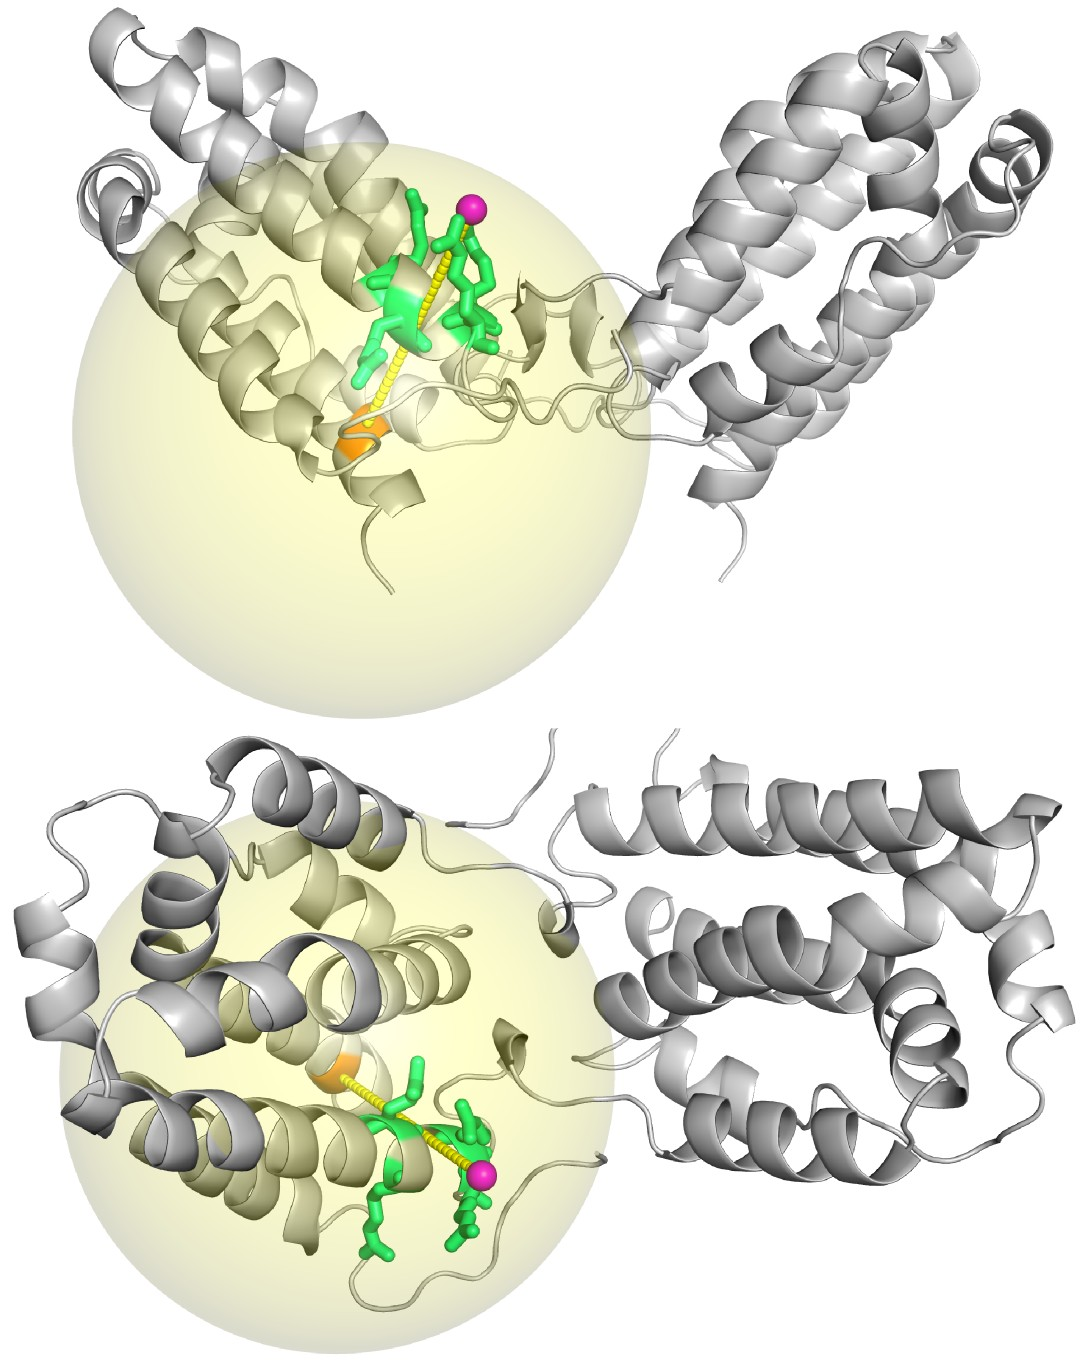
\includegraphics[width=1.0\textwidth]{gfx/dmdil10/round1_il10_ligandcenter_proteincore_sphere_top_and_side_001.jpg}
\caption[]{Geometrical DMD parameterization used for most of the DMD studies
in the first stage. The IL-10 dimer is shown in gray ribbon representation (top:
side view on the V-shape, bottom: top-down view on the V-shape). The C-alpha
atom of methionine 154 in the human interleukin-10 sequence was selected as
protein core atom (ribbon colored in orange). The focus point (small sphere
colored in magenta) was selected manually based on the putative binding region
comprised by residues R102, R104, R106, R107 (colored in green sticks). The tMD
target distance of \SI{17.7}{\angstrom} between the protein core atom and the
focus point is indicated by a thick yellow dashed line. The large transparent
yellow sphere is centered on the protein core atom and its radius is set to the
tMD target distance (after tMD, all central ligand atoms are located on that
spherical surface).}
\label{fig:dmdil10:dmd_geometry_round1}
\end{figure}

\Cref{fig:dmdil10:dmd_geometry_round1} visualizes the geometrical DMD
parameterization used for most of the DMD studies in the first stage. The manual
selection of core atom and focus point was based on the binding site prediction
made by Coulomb potential analysis (see \cref{bspred:il10}) and performed in
compliance with the guidelines formulated in \cref{dmd:lrom_preparation}. The
C-alpha atom of M154 was selected as core atom. The tMD target distance was set
to \SI{17.7}{\angstrom}, yielding a quite large spherical surface for proper
putative binding site sampling.

% If relevant, deviations from this geometrical
%setup in the first or second stage of DMD studies are described in the results
%and discussion part.

\subsubsection{DMD result consistency}

One of the first observations in this stage of DMD studies was method
consistency, i.e.\ further support for sufficient sampling and convergence of
the DMD method. \Cref{fig:dmdil10:hp_hexa_vs_tetra_clusters_position_match}
shows the overlay of two clustering results from two independently performed DMD
studies that differed only in the GAG ligand length --- one was performed with a
heparin hexasaccharide, and the other with a heparin tetrasaccharide. Ideally,
one would want DMD to return a very similar binding pose prediction in both
cases, as it is unlikely for these two GAG molecules to behave fundamentally
different. As motivated in \cref{relevance_of_clustering}, comparison of the
position of the most populated clusters in both cases is a way to (in)validate
this assumption. Note that comparison of both clusters, and with that,
comparison of both DMD studies with respect to the distribution of docking
solutions, is only possible because great care was taken of making both
clustering results comparable via the clustering parameter optimization
described in \cref{clustering_param_opt}. In both cases, the docking solution
clustering was performed with $N_{min}$ (the minimal number of clusters that
must be found) set to 1, and $M_{min}$ (the minimal number of members within
each cluster) set to 4. In both cases, the automatic clustering parameter
optimization yielded an $\epsilon$ value of \SI{2.6}{\angstrom}, i.e.\ just
about the same density of docking solutions in both clusters.

\begin{figure}
\centering
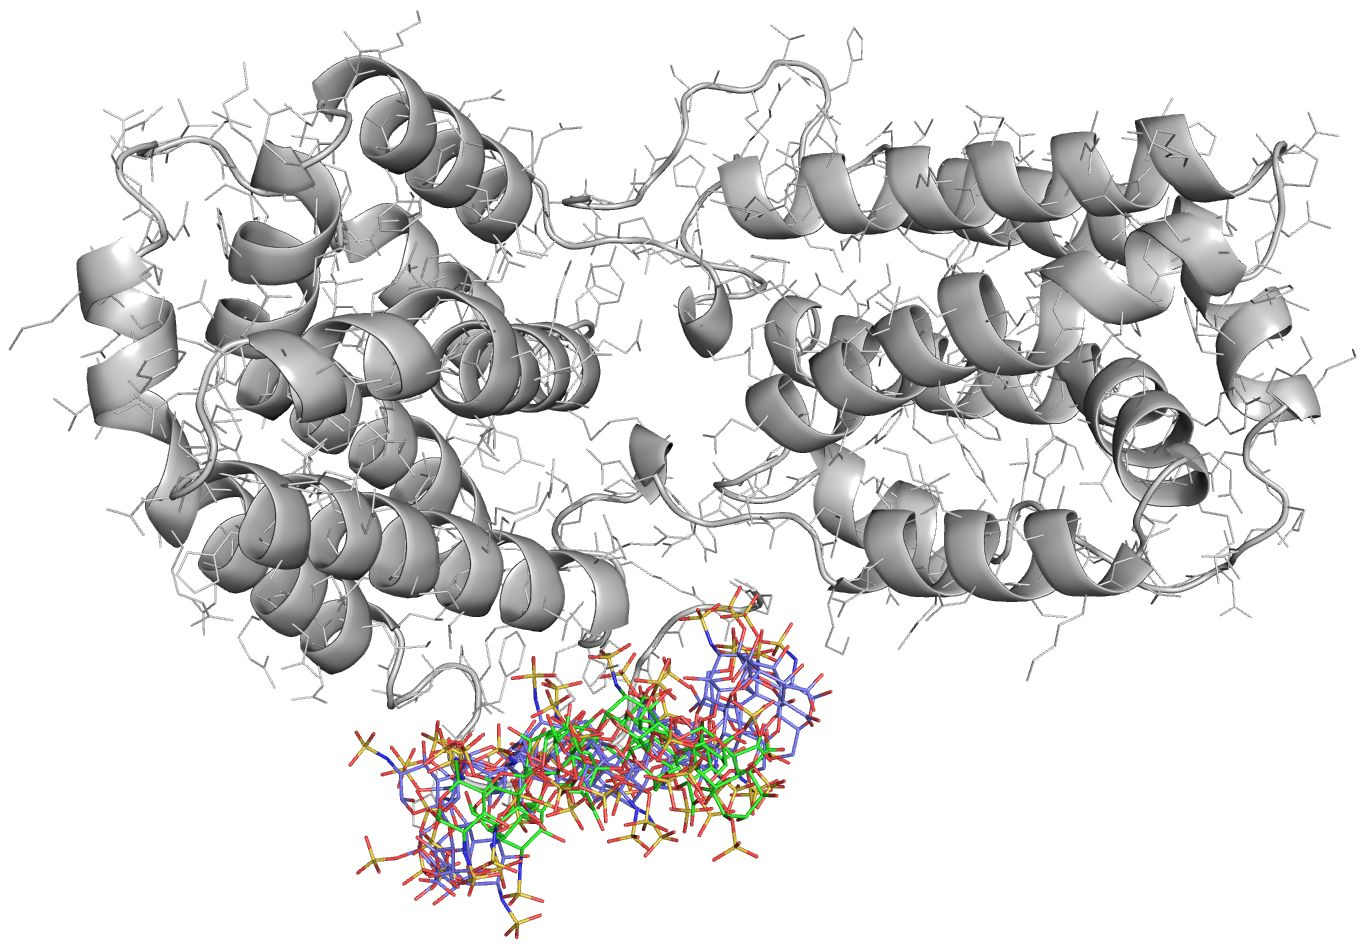
\includegraphics[width=1.0\textwidth]{gfx/dmdil10/hp_hexa_vs_tetra_clusters_position_match_cropped.jpg}
\caption[]{Consistent results among two independently conducted DMD studies.
Setup and protocol of both DMD studies differed only in the GAG ligand length,
one was performed with a heparin hexasaccharide, the other with a heparin
tetrasaccharide. The most populated cluster of docking solutions derived from
the hexasaccharide study is shown with carbon atoms in blue, and the
corresponding tetrasaccharide representation is shown with carbon atoms in
green. The IL-10 structure (PDB ID 2ILK) is shown in gray cartoon/line
representation.}
\label{fig:dmdil10:hp_hexa_vs_tetra_clusters_position_match}
\end{figure}

In essence, both clusters are positioned equivalently with respect to IL-10, and
show the same density. That is, with respect to the distribution of docking
solutions, both DMD studies returned the same result. In addition to the DMD
validation study presented in \cref{chapter:dmd}, this proves the significance
of data created by the DMD method.


\subsubsection{Impact of N-terminal residues and modest geometry changes}
%NOTE: when changing this heading, also change the "quote" in the section
% \subsubsection{Ensemble-derived single-residue energy decomposition} below.

In one of the early studies, the five N-terminal residues of IL-10 (see
\ref{dmdil10:overallmethod}) were included, and the geometrical parameterization
of DMD was varied compared to the setup described in
\ref{dmdil10:method_geom_setup_1st}: the C-alpha of M154 was kept as core atom, but
the focus point was changed slightly within the anticipated binding region,
resulting in a different orientation of the yellow axis shown in
\cref{fig:dmdil10:dmd_geometry_round1}, and in a tMD target distance of
\SI{20.5}{\angstrom} instead of \SI{17.7}{\angstrom}. The rest of the system and
protocol setup was equivalent to another DMD study (both incorporated a heparin
tetrasaccharide as ligand molecule), whose geometrical outcome is shown in
\cref{fig:dmdil10:hp_hexa_vs_tetra_clusters_position_match}. As it turned out,
the final distribution of docking solutions was not affected by the changes: the
location of the most populated clusters of both DMD studies matched

% (the
%position of one of the clusters is shown in
%\cref{fig:dmdil10:hp_hexa_vs_tetra_clusters_position_match}).

It can be concluded that the main data obtained from a DMD study are rather
insensitive with respect to modest changes in the geometrical parameterization
of DMD, and that the presence of the five N-terminal residues does not
significantly affect the DMD binding pose prediction, i.e.\ the assumption from
here on is that the flexible part of IL-10's N-terminus can be neglected for
investigating the main mechanism of IL-10-GAG interaction.


\subsubsection{Distinction of GAG types by cluster statistics}

\begin{table}
\footnotesize
\centering
\renewcommand{\arraystretch}{1.3}
\begin{tabular}{lcrll}
\midrule
GAG type                 & cluster members & $\epsilon$ (\si{\angstrom}) & $m$ (\si{\angstrom}) & $\Delta G$ (\si{\kilo\calory\per\mol}) \\
\midrule
HP dp6                   & 4               & 2.5                         & 2.8 $\pm$ 0.7          & -45 $\pm$ 15                           \\
CS4 dp6                  & 5               & 3.2                         & 2.6 $\pm$ 0.3          & -37 $\pm$ 8                            \\
CS4 dp6 (2nd cluster) & 4               & 3.2                         & 2.4 $\pm$ 0.4          & -37 $\pm$ 14                          \\
\midrule
\end{tabular}
\caption{
Characterization of most populated clusters by single-run quantity cluster
statistics for two different DMD studies differing only in the GAG type. In one
study, a HP dp6 was used as ligand, in the other study a CS4 dp6 was used. The
HP study yielded a single prominent cluster, the CS4 study yielded two similar
clusters. $\epsilon$ is the spatial density of docking solutions according to
\cref{clustering_param_opt}. $m$ is the mobility of the ligand relative to the
receptor, as defined in \cref{dmd:dataanalysis}. Here, $\Delta G$ is the free
energy of binding estimate as provided by the MM-PBSA method
(\cref{methods:mmpbsa_mmgbsa}). The standard deviations shown are derived from
the cluster-internal variations.}
\label{tab:dmdil10:round1_different_gag_types}
\end{table}

Ideally, different behavior of different GAG types is manifests itself in the
docking solution clustering, and especially in the single-run quantities
evaluated on a per-cluster basis. The characterization of most populated
clusters for two different DMD studies differing only in the GAG type should be
discussed by means of an example. In one study, a heparin (HP) hexasaccharide
was used, in another study a chondroitin-4-sulfate (CS4) hexasaccharide was
used. The heparin study yielded a single prominent cluster, the CS4 study
yielded two almost equally populated clusters. The placement of all clusters
relative to IL-10 was similar, and the quantitative evaluation of the clusters
yielded similar results (see
\cref{tab:dmdil10:round1_different_gag_types}): among the three clusters, the
ligand movement relative to the receptor as well as the MM-PBSA free energy of
binding estimate are indistinguishable, considering the cluster-internal
fluctuations represented by the standard deviations. Just the cluster density
indicates that the docking solutions obtained for HP show a little more spatial
consistency than the solutions obtained for CS4.

The important conclusion to be drawn from this (and analogous observations) is
that the IL-10-GAG system does not easily allow for a binary distinction of
different GAG types via DMD with respect to their interaction \enquote{mode}.
From the DMD studies performed until here, different GAG types seem to yield
data from a continuous spectrum, showing at most quantitative differences, but
no qualitative differences in their behavior. Likewise, if there is binding
specificity of IL-10 for a certain GAG type, it remained undetectable with the
kind of data acquisition and analysis performed so far.

\subsubsection{Ensemble-derived hydrogen bonding information}

\begin{figure}
\centering
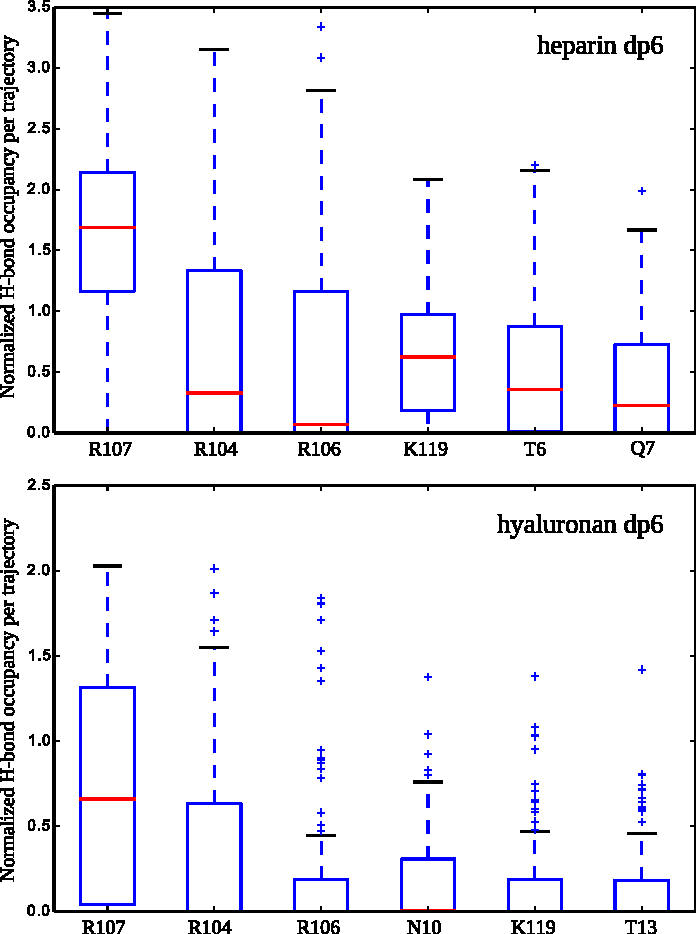
\includegraphics[width=1.0\textwidth]{gfx/dmdil10/round1_il10_hbond_hadp6_vs_hpdp6.pdf}
\caption[]{Most important residues of IL-10 for GAG-interaction, as identified
by DMD ensemble-derived hydrogen bonding information, from two independently
performed DMD studies differing \textit{only} in the GAG type (top: heparin
hexasaccharide, bottom: hyaluronan hexasaccharide). The box plot representation
is made from  $N=100$ samples per box, whereas each sample is the number of
hydrogen bond donors integrated and normalized over the data production period
of one free MD trajectory, for the residue specified in the abscissa label.
The residues are sorted by the \textit{mean} (not shown), the red bars indicate
the \textit{median} (close to zero if not visible).}
\label{fig:dmdil10:hp_hexa_vs_ha_hexa_hbond}
\end{figure}


As explained in the \enquote{extraction of ensemble properties} part of
\cref{dmd:dataanalysis}, a DMD study is able to yield reliable information
about the importance of single receptor amino acids for ligand binding, via
e.g.\ hydrogen bonding (H-bond) analysis of the MD trajectory data.
Surprisingly, all of the DMD studies performed in the first stage of studies
returned the same clear and unequivocal result --- that R107 of IL-10 plays a
major role in IL-10-GAG interaction. \Cref{fig:dmdil10:hp_hexa_vs_ha_hexa_hbond}
shows ensemble-derived H-bond information for two independently performed DMD
studies differing in the GAG type: one was performed with a HP dp6, the other
with a HA dp6. For each free MD trajectory in these two DMD studies the
normalized occupancy of H-bond donor atoms in each receptor residue was
determined, and the results were ranked by the mean normalized occupancy. All
donors within single residues were accumulated; for instance an arginine can
donate up to three hydrogens at the same time (the maximum normalized occupancy
in this case would be 3). \Cref{fig:dmdil10:hp_hexa_vs_ha_hexa_hbond} shows the
top six H-bond-donating residues for both studies, including box plot
representations of the corresponding distributions. In both cases, R107 is
ranked first by mean as well as median. In case of HP dp6, a mean R107 occupancy
of about 1.7 was measured, i.e.\ throughout the entire DMD study this residue
donated (on average) almost \textit{two} hydrogen atoms to different hydrogen
bond formations. This number alone is a strong indicator for the relevance of
this residue in protein-GAG interaction. However, the essential observation is
that R107's hydrogen bonding properties qualitatively stand out compared to the
other amino acid in IL-10: the H-bond occupancy distributions of all other
residues have their maximum near 0, and a decay towards higher occupancies,
yielding a median close to 0, in both cases shown (HP dp6 and HA dp6). The
occupancy distribution of R107, however, has a median clearly far from 0. In
case of HP dp6, the distribution has its global maximum at about 1.5. It can be
concluded that most of the molecular surface of R107 is solvent-exposed, and
significantly more accessible for interaction with functional groups of GAGs
than the other residues.

Hyaluronan has significantly less functional groups (carboxyls and sulfates)
available that might act as H-bond acceptors than heparin. Quantitatively, this
difference is clearly reflected in the mean value of the H-bond occupancy
distributions, with about 1.7 for HP dp6 and about 0.7 measured for HA dp6. For
all different GAG types and lengths investigated in the first stage of IL-10-GAG
DMD studies (CS4 dp4, CS6 dp4, HA dp4, HP dp4, figures not shown for all GAG
types), R107 showed distinct behavior by the quantitative and qualitative
criteria described in the paragraph above. A clear conclusion is that R107
significantly stands out compared to all other residues and supposedly plays a
particularly important role in IL-10- GAG recognition.

\subsubsection{Ensemble-derived single-residue energy decomposition}

\begin{figure}
\centering
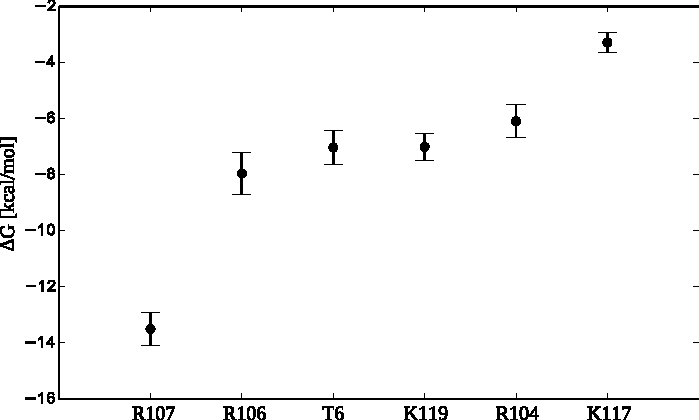
\includegraphics[width=0.97\textwidth]{gfx/dmdil10/round1_il10_SRED_hpdp6.pdf}
\caption[]{Merged single-residue energy decomposition (SRED) data from a
DMD study with a HP dp6 ligand. The DMD study was comprised of 200 runs. The
SRED data of the top \SI{40}{\percent} of the DMD runs ranked by MM-PBSA
$\Delta G$ were merged into the data points shown. The error bars represent the
standard error of the mean.}
\label{fig:dmdil10:SRED_hpdp6}
\end{figure}

I have observed the ensemble-merged MM-GBSA single-residue energy decomposition
(SRED, as explained in the \enquote{extraction of ensemble properties} part of
\cref{dmd:dataanalysis}) data to yield results generally consistent with those
of the hydrogen bonding analysis. Most importantly, the SRED data also points
out the importance of R107 for IL-10-GAG recognition.
\Cref{fig:dmdil10:SRED_hpdp6} shows the six top-ranked IL-10 residues according
to SRED performed on a DMD study with a HP dp6. In this case, the DMD study was
comprised of $N=200$ DMD runs, and the SRED data of the top \SI{40}{\percent} of
the DMD runs according to the MM-PBSA free energy of binding estimate has been
merged, yielding 80 DMD runs contributing to the data shown. The error bars
represent the standard error of the mean, and one can conclude that ---
considering the statistical error --- the residues on ranks two to five are not
distinguishable, ranging in the interval between \SI{-6}{\kilo\calory\per\mol}
and \SI{-8}{\kilo\calory\per\mol}. R107, however, has a special role, with a
significantly stronger mean interaction energy of \SI{-13.5 +-
0.5}{\kilo\calory\per\mol}. Note that the absolute values of these energies as
well as the inter-residue energy distance are not meaningful. The relative
distances, however, yield resilient information. As in case of hydrogen bonding
data, those DMD studies in the first stage of studies differing from the
above-described setup in GAG type and length also revealed R107 as having the
strongest interaction with the GAG, leaving all other residues far behind (data
not shown).

Further insights were derived from the SRED data obtained from the IL-10-GAG DMD
studies in the first stage. For instance, the DMD study with a HA dp6 used as
ligand led to the same qualitative SRED results as discussed in the paragraph
above, in the sense that R107 stood out. However, the corresponding mean
interaction energy was determined as \SI{-3.8 +-0.3}{\kilo\calory\per\mol},
which is about \SI{70}{\percent} weaker than in case of the HP dp6 study.
Qualitatively this drop is expected as of the fewer sulfate groups in HA
compared to HP. Also, the observation is in compliance with the hydrogen bonding
data discussed in the previous section, where we observed a drop of about
\SI{60}{\percent} in the R107 hydrogen bond occupancy when changing from heparin
to hyaluronic acid.

In general, it can be concluded that both, SRED and hydrogen bonding analysis
are able to identify R107 as especially important, whereas the hydrogen bonding
analysis is computationally less complex than SRED. Furthermore, both types of
analyses can quantitatively express the effect of a drop in the number of
sulfate groups per repeating GAG unit. Another interesting observation made is
that inclusion of IL-10's N-terminus does not significantly influence the
outcome of SRED as well as hydrogen bonding data, in line with the conclusions
drawn in the \enquote{Impact of N-terminal residues and modest geometry changes}
part above.



\subsubsection{Mutating IL-10's arginine 107 to alanine}

\begin{figure}
\centering
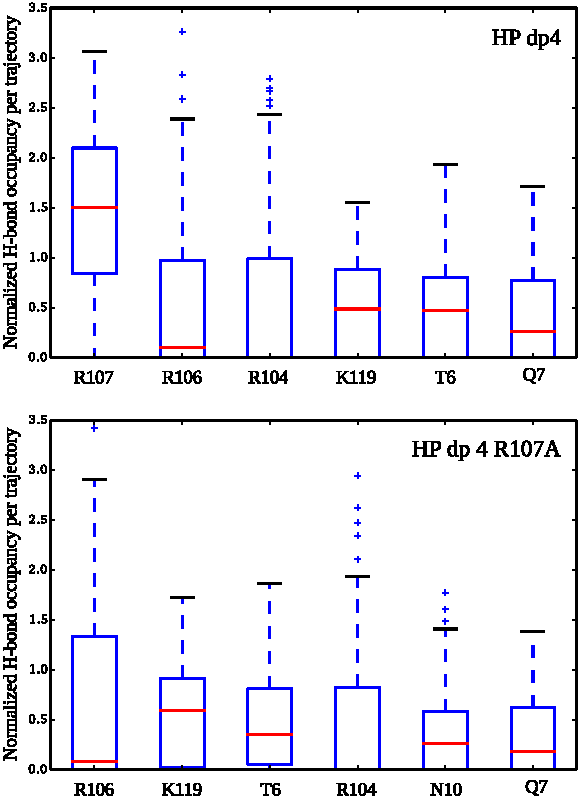
\includegraphics[width=1.0\textwidth]{gfx/dmdil10/first_stage_Hbonding_hp_dp4_R107A_vs_unmutated.pdf}
\caption[]{Most important residues of IL-10 for GAG-interaction, as identified
by ensemble-derived hydrogen bonding information from two independently
performed DMD studies using a HP dp4 ligand, and differing only in the IL-10
sequence at position 107. Top: canonical human IL-10 sequence. Bottom: R107A
mutation. The box plot representation is made from $N=100$ samples per box,
whereas each sample is the number of hydrogen bond donors integrated and
normalized over the data production period of one free MD trajectory, for the
residue specified in the abscissa label. The residues are sorted by the
\textit{mean} (not shown), the red bars indicate the \textit{median} (close to
zero if not visible).}
\label{fig:dmdil10:hpdp4_normal_vs_R107A}
\end{figure}

Up to here, various observations have been made, independently suggesting that
R107 has an important role in IL-10-GAG interaction. For further characterizing
the impact of this residue, a DMD study was performed with an R107A mutation of
the IL-10 sequence while keeping all other parameters equivalent to another
study performed before, both using a HP dp4 molecule as ligand. The most
concrete observation from this comparison stems from hydrogen bonding and SRED
analysis. No other amino acid residue was able to compensate the loss of the
polar and hydrogen bonding properties of R107, not even its neighboring
arginines: with the R107A mutation, the hydrogen bond occupancy of the
non-mutated residues did almost not change, as shown in
\cref{fig:dmdil10:hpdp4_normal_vs_R107A}. The box plot representations of the
hydrogen bonding occupancy of R104, R106, and K119 indicate similar behavior in
both studies. Particularly, the box plot representation of the hydrogen bonding
occupancy of R107 in the non-mutated IL-10 finds no resemblance in the DMD study
with the mutant protein. The SRED analysis for the non-mutated system yielded an
interaction energy of
\SI{-13.5 +- 0.8}{\kilo\calory\per\mol} for R107, leaving all other residues far
behind, and R106 was assigned an energy of \SI{-5.5 +-
0.8}{\kilo\calory\per\mol}. In contrast, the SRED analysis for the mutated
system ranked R106 first, with an interaction energy of \SI{-8 +-
1.0}{\kilo\calory\per\mol}, indicating a weak compensation effect, in the sense
that R106 becomes slightly more important for GAG-binding in case of the R107A
mutation. However, also the SRED analysis reveals that the qualitative nature of
the interaction between R107 and the tested GAG molecules can not be reproduced
by any other amino acid in that region, supporting the picture in which R107
takes a \textit{unique} role for IL-10-GAG interaction. All in all, these
observations further corroborate the importance of R107 for IL-10-GAG
interaction.


\subsection{2nd stage of DMD studies}


\subsubsection{Optimized DMD parameterization}
\label{dmdil10:method_setup_2nd}

In the second stage of IL-10-GAG DMD studies, the geometrical parameterization
was chosen based on the docking solution clustering results obtained in the
first stage. There, the most populated clusters of docking solutions were mostly
located in the same place, positioned very similar to the clusters shown in
\cref{fig:dmdil10:hp_hexa_vs_tetra_clusters_position_match}.  Following the
paradigm of the iterative method for obtaining convergence, the DMD focus point
was aligned towards this agglomeration of DMD docking solutions, in order to
further focus the sampling onto that region: the new focus point was set onto
the central atom of a representative docking solution from above-mentioned
clusters. The C-alpha atom of M154 was kept as core atom, yielding a tMD target
distance of \SI{20.5}{\angstrom}.

An optimization implemented in the second stage of DMD studies was the reduction
of the target displacement length for the LROM setup. It was shortened from
\SI{30}{\angstrom} to \SI{25}{\angstrom}, effectively decreasing the system size
and therefore the computational effort for performing the tMD simulations.
Furthermore, the tMD simulation time was decreased from \SI{4}{\nano\second} to
\SI{3}{\nano\second}. Overall, 98 DMD runs were completed for CS4 dp6, 200 runs
for CS6 dp6, 198 runs for HA dp4, 278 runs for HA dp6, 194 runs for HP dp4, and
298 runs for HP dp6.


\subsubsection{SRED results}


\begin{figure}
\centering
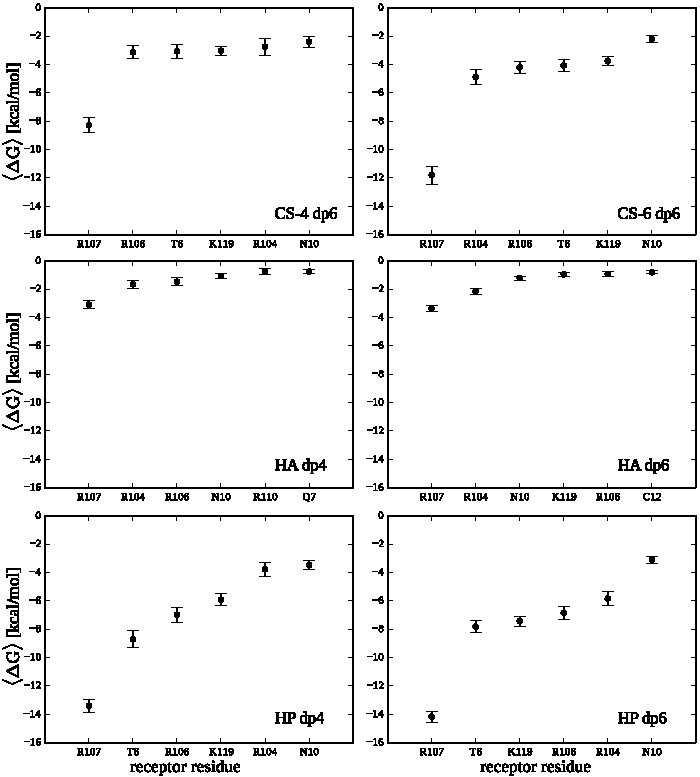
\includegraphics[width=1.0\textwidth]{gfx/dmdil10/second_stage_all_SREDs_05.pdf}
\caption[]{
Merged single-residue energy decomposition (SRED) data for six independently
performed DMD studies differing only in the type of ligand, as indicated in the
right bottom corner of each plot. The data shown stems from 98 DMD runs
completed for CS4 dp6, 200 runs for CS6 dp6, 198 runs for HA dp4, 278 runs for
HA dp6, 194 runs for HP dp4, and 298 runs for HP dp6. The SRED data of the top
\SI{40}{\percent} of the DMD runs ranked by MM-PBSA $\Delta G$ were merged into
the data points shown. The error bars represent the standard error of the mean.
}
\label{fig:dmdil10:2nd_stage_all_SREDs}
\end{figure}

\Cref{fig:dmdil10:2nd_stage_all_SREDs} shows all SRED results obtained from the
second stage of DMD studies. Again, R107 ranks first in all studies.
Qualitatively, for all GAG types containing sulfate groups (not HA), there is a
clear separation between R107 and the residues ranked second or worse. Ranks two
to six are not well-resolved in all cases, considering the error bars which
represent the statistical error of the method. Quantitatively, the energetic
contribution of single amino acid residues is shown to be much larger for
sulfated GAGs than for HA. In these lines, the observations obtained from the
first stage of DMD studies are reproduced.

Another observation is that for HP as well as for HA, which have both been
analyzed as dp4 and dp6 variants, there is no significant difference in the SRED
result depending on the length of the GAG. That is, at least within the scope of
the methodology used here, tetra- and hexasaccharides are identified to show
qualitatively the same behavior.

An important observation is that the set of the top six residues obtained from
SRED in the second stage of studies is the same for all sulfated GAG types
(i.e.\ for HP, CS4 and CS6): R107, R106, R104, K119, T6, N10. This is another
evidence for the convergence of the DMD method and its subsequent data analysis.
Additionally, this expresses that the resides ranked two to six --- while their
internal ranking might be unclear --- have not been identified as important by
coincidence (noise), but arguably actually contribute more to GAG binding than
other residues not listed in the top six. When the set of top six residues
identified for the sulfated GAG types is compared to the binding region
prediction made in \cref{chapter:bspred}, one notes that R102 does not appear in
any of the top six rankings. That R102 does not appear here might be due to the
localized nature of the DMD method, and it could be that the location bias
introduced via the geometrical DMD parameterization does not allow R102 to be
properly sampled by the ligand. However, since R102 is spatially so close to
R106 and R107, I tend to conclude that R102 actually \textit{is} less important
for GAG binding than initially assumed just based on the Coulomb potential
distribution. A notable observation in this context is the importance of T6,
which might actually be an artifact: in all second stage DMD studies, T6 is the
N-terminal residue of IL-10, and therefore it is quite accessible for the
ligand, whereas in reality it is not the terminus.

Regarding the DMD method itself, one can conclude that the reduction of the
target displacement length to \SI{25}{\angstrom} and the reduction of pulling
process simulation time to \SI{3}{\nano\second} did not lead to observable
caveats --- in fact, the results described so far from the second stage of DMD
studies are in compliance with those DMD results obtained in the first stage of
studies.


\subsubsection{Docking solution clustering}


\begin{figure}
\centering
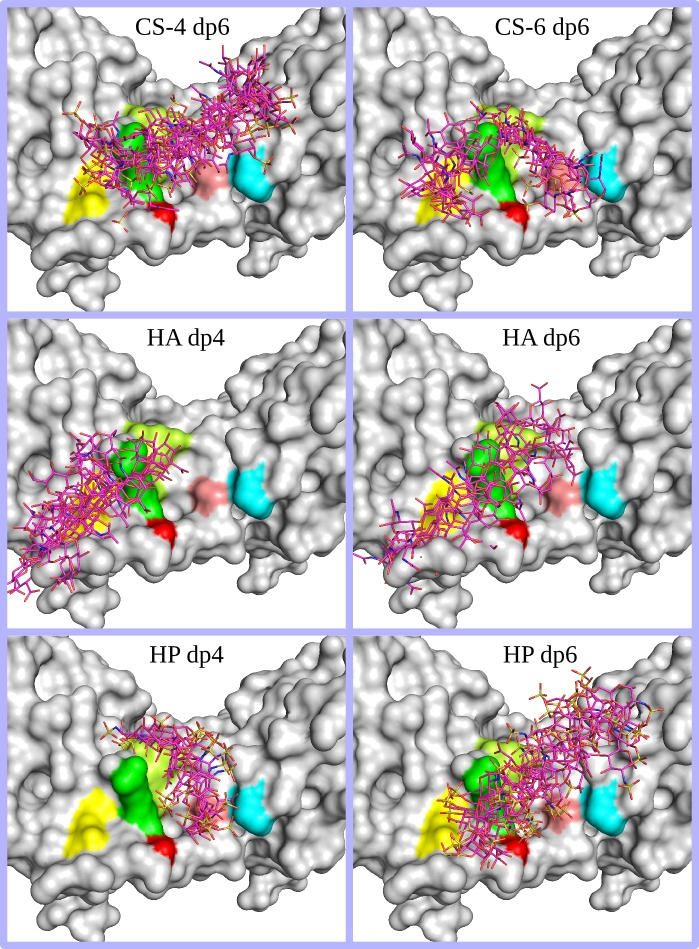
\includegraphics[width=1.0\textwidth]{gfx/dmdil10/2ndstage_allclusters_04.jpg}
\caption[]{
Most populated docking solution clusters of all second stage DMD studies,
obtained with a consistent approach. The studies differ only in the GAG type and
length (as defined in the panel headings). The GAG structures within each
cluster are shown with carbon atoms in magenta. The IL-10 structure (PDB ID
2ILK) is shown in gray surface representation. The surface of the reproducibly
obtained top six set of residues according to the ensemble-derived SRED analysis
is colorized: R107 in green, R106 in light green, R104 in yellow, K119 in
cyan, N10 in red, and T6 in light red.}
\label{fig:dmdil10:2nd_stage_all_clusters}
\end{figure}



\Cref{fig:dmdil10:2nd_stage_all_clusters} shows the most populated docking
solution clusters for all second stage DMD studies. In all cases, the clustering
was performed with $N_{min}$ (the minimal number of clusters that must be found)
set to 1, and $M_{min}$ (the minimal number of members within each cluster) set
to 5, i.e.\ the clustering results are comparable (see \cref{chapter:clustering}
for details). There are a couple of important observations to be made from these
data. First of all, there are two principally different GAG binding orientations
found, both heavily involving R107. From the point of view shown in
\cref{fig:dmdil10:2nd_stage_all_clusters}, one principal binding pose is
oriented from the bottom left to the upper right, with the GAG being placed in a
IL-10 surface groove below R107. This is true for CS4 dp4, for both HA
scenarios, and for HP dp6. A second qualitatively different pose is oriented
from the top left to the bottom right, with the GAG placed above R107, and
squeezed between R107 and K119 (shown in green and cyan in the figure,
respectively). This is true for the HP dp4 scenario. The structures in the CS6
dp6 cluster are bent in a way that they can be considered a combination of both
principal binding poses. \Cref{fig:dmdil10:2nd_stage_principal_poses} visualizes
both principally different poses schematically.

\begin{figure}
\centering
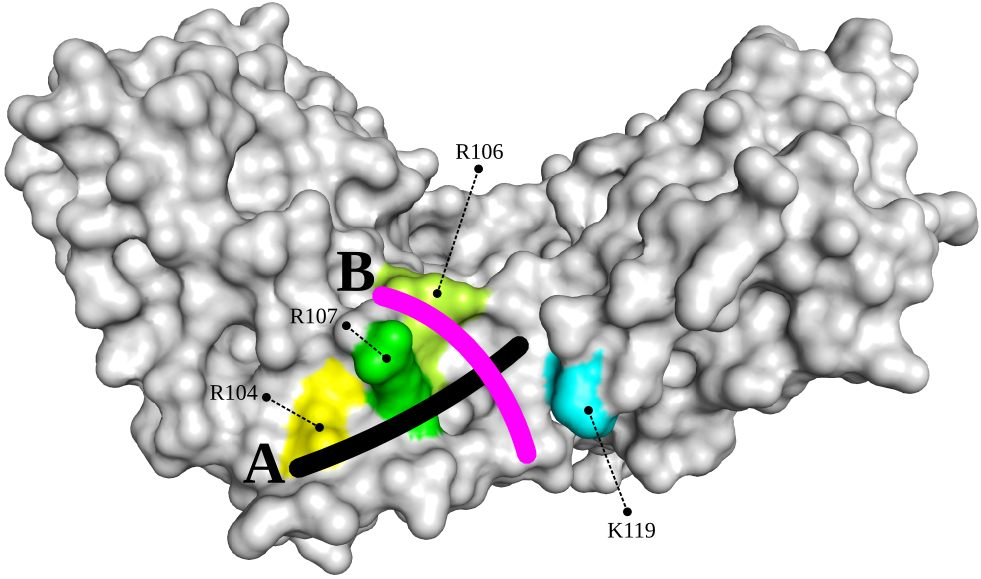
\includegraphics[width=1.0\textwidth]{gfx/dmdil10/principal_poses_06.jpg}
\caption[]{
Schematic visualization of two principally different GAG binding poses observed
via docking ensemble clustering of all second stage DMD studies. Pose A
(indicated in black) has the GAG placed in a IL-10 surface groove right
\enquote{below} R107 (from the point of view shown here). Pose B (indicated in
magenta) has the GAG placed above R107 and within the groove between R107 and
K119. The IL-10 structure (PDB ID 2ILK) is shown in gray surface representation.
The four positively charged residues being most important for GAG binding
(according to ensemble-derived SRED analysis) are labeled and their surface is
colorized.}
\label{fig:dmdil10:2nd_stage_principal_poses}
\end{figure}

It is notable that there actually is a qualitative difference for the cluster
poses obtained for HP dp4 and HP dp6. This is not supported by the SRED data
described in the section before, where it was found that HP tetra- and
hexasaccharides show qualitatively the same behavior. This is not \textit{per
se} a contradiction, since the SRED data represent a large ensemble of docking
solutions, while clustering explicitly selects a small fraction of the ensemble,
under the assumption that this fraction represents the most probable state.
However, since the clustering method introduces assumptions and approximations
on top of the DMD approach --- which increases the overall uncertainty --- the
SRED ensemble data is more reliable than the clustering result. Therefore, as of
a lack of support from the SRED data, none of both principal binding
orientations discussed above must be excluded for both, HP dp4 and dp6.

Looking at the structure ensembles shown in
\cref{fig:dmdil10:2nd_stage_all_clusters} it makes sense that K119 has been
identified (via SRED) as being a strong contributor to GAG binding: the groove
between R107 and K119 could serve as a trap, potentially anchoring a GAG from
two sides simultaneously, with a positively charged amino acid residue on both
sides. The groove is just wide enough for e.g.\ heparin, as can be seen in the
HP dp4 panel of \cref{fig:dmdil10:2nd_stage_all_clusters}. The clustering data
can be used for characterizing the GAG binding properties of this groove: the HP
dp4 cluster (which is located in mentioned groove) shows the highest structural
consistency among all clusters shown in
\cref{fig:dmdil10:2nd_stage_all_clusters}. The similarity among the structures
in this cluster has been quantified with $\epsilon = \SI{2.2}{\angstrom}$ (this
value actually encodes the \enquote{density-reachabiltiy}, and the smaller the
value, the larger the similarity; see \cref{chapter:clustering} for details).
This structural consistency is significantly larger than in the other cases (HP
dp6: $\epsilon = \SI{2.6}{\angstrom}$, HA dp4: $\epsilon = \SI{3.0}{\angstrom}$,
HA dp6: $\epsilon = \SI{2.6}{\angstrom}$, CS4 dp6: $\epsilon =
\SI{3.4}{\angstrom}$, CS6 dp6: $\epsilon = \SI{2.7}{\angstrom}$). Presumably,
the reason for this comparably large structural consistency is that heparin
tightly fits into this groove, with less conformational freedom when compared to
the other binding modes shown in \cref{fig:dmdil10:2nd_stage_all_clusters}.



N=200 and N=300 for much clearer clustering and reduction of target displacement
length to 25 Angstroms and pulling process simulation time to 3 ns instead of 4
without observable caveats.

Compare cluster positions to those residues that appear over and over again in
top rankings. Is there a correspondence?


Note which residues appear over and over in top rankings: R107, 106, 104,
compare with binding region prediction in chapter X. Is there an additional hot
candidate? K119? Is there one listed in the prediction that does not appear
to be THAT important?



\hl{Note (TODO):}
Show picture of R107 specifically marked in the structure, together with
crystal sulfates, discuss possible binding poses involving these crystal
sulfates. Nee, mach das später, bei bringing it all together.





\subsection{Conclusions}

\hl{Note (TODO):}
So far, about 10 independent DMD studies involving IL-10 and different GAGs
have been performed. An important intermediate result of the corresponding data
analysis is that one amino acid residue, R107 (in the hIL-10 sequence, conserved
in mouse), significantly stands out compared to all other residues and
supposedly plays a particularly important role in IL-10-GAG recognition. This
conclusion is based on different types of data, including time-averaged hydrogen
bonding analysis and single-residue energy decomposition applied to MD data
collected on the microsecond time scale.

